\chapter{Proposed Framework}
As it has shown, one of the main task of predictive maintenance is Anomaly Detection, described as a set of techniques for the identification of some anomalous warning states in which an under observation machine could be, allowing a better maintenance activities planning. In this part of the work the task performed is firstly formalized and then the proposed architecture is illustrated. At the end of the chapter there is a brief explanation of the technologies used for the implementation of the illustrated framework.
\section{Problem definition}
In this section the performed anomalous sound detection task is formalized. The proposed architecture must learn to classify audio clips placed in input as normal or anomalous. The training set is composed by $K$ audio clips $\{x_1, x_2, ...,x_K\}$ in \textit{.wav} format, recorded from different kinds of a machine $M$, with a duration of $T$ seconds. An ID string is used to identify the different kinds of $M$. The main goal of this problem is to train a model on all clips that belong to normal working state of $M$ and, since only few audio clips are recorded when anomalies are present, they are incorporated into a different set, used for testing purpose. For the reasons explained in previous chapters, this task cannot be solved as a simple classification problem, even though it seems to be a two-class classification problem.\\
Before describing the proposed model in detail, let’s have a look to the implemented framework in high level way (Figure \ref{high-level-architecture}). As it can be seen, the input consists in an audio clips recorded by microphones disposed around the monitored machinery, while the output is a label, \textit{normal} or \textit{anomaly}.
\begin{figure}[ht]
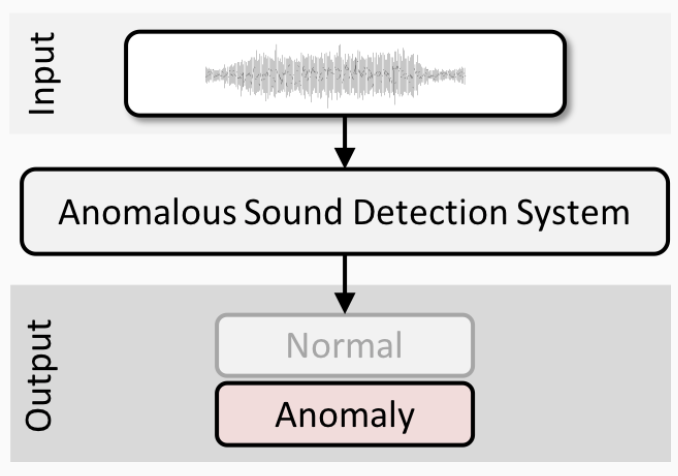
\includegraphics[scale=0.95]{TESI DI FIORE/img/high-level-architecture.png}
\centering
\caption{High level architecture \cite{DCASE}}
\label{high-level-architecture}
\end{figure}

\section{Model architecture}
The proposed ASD system shown in Figures \ref{offline-asd-system} and \ref{online-asd-system} consists of two main phases: an offline phase, responsible of the training of an autoencoder model and an online operation phase to conduct the ASD in real time. It is good to say immediately that this architecture is valid for different implementations of the autoencoder component. In fact, the novelty brought by this work is a generalization of ID embedding idea, shown in Chapter 2 and implemented for DCASE 2020 task 2 Dataset, through the use of different kinds of autoencoders, in terms of how the encoder or the decoder layers are built.\\
In the next two subsections there are detailed descriptions of the two phases, with a focus on each block present in the pipelines.
\subsection{Offline Training Phase}
\begin{figure}[ht]
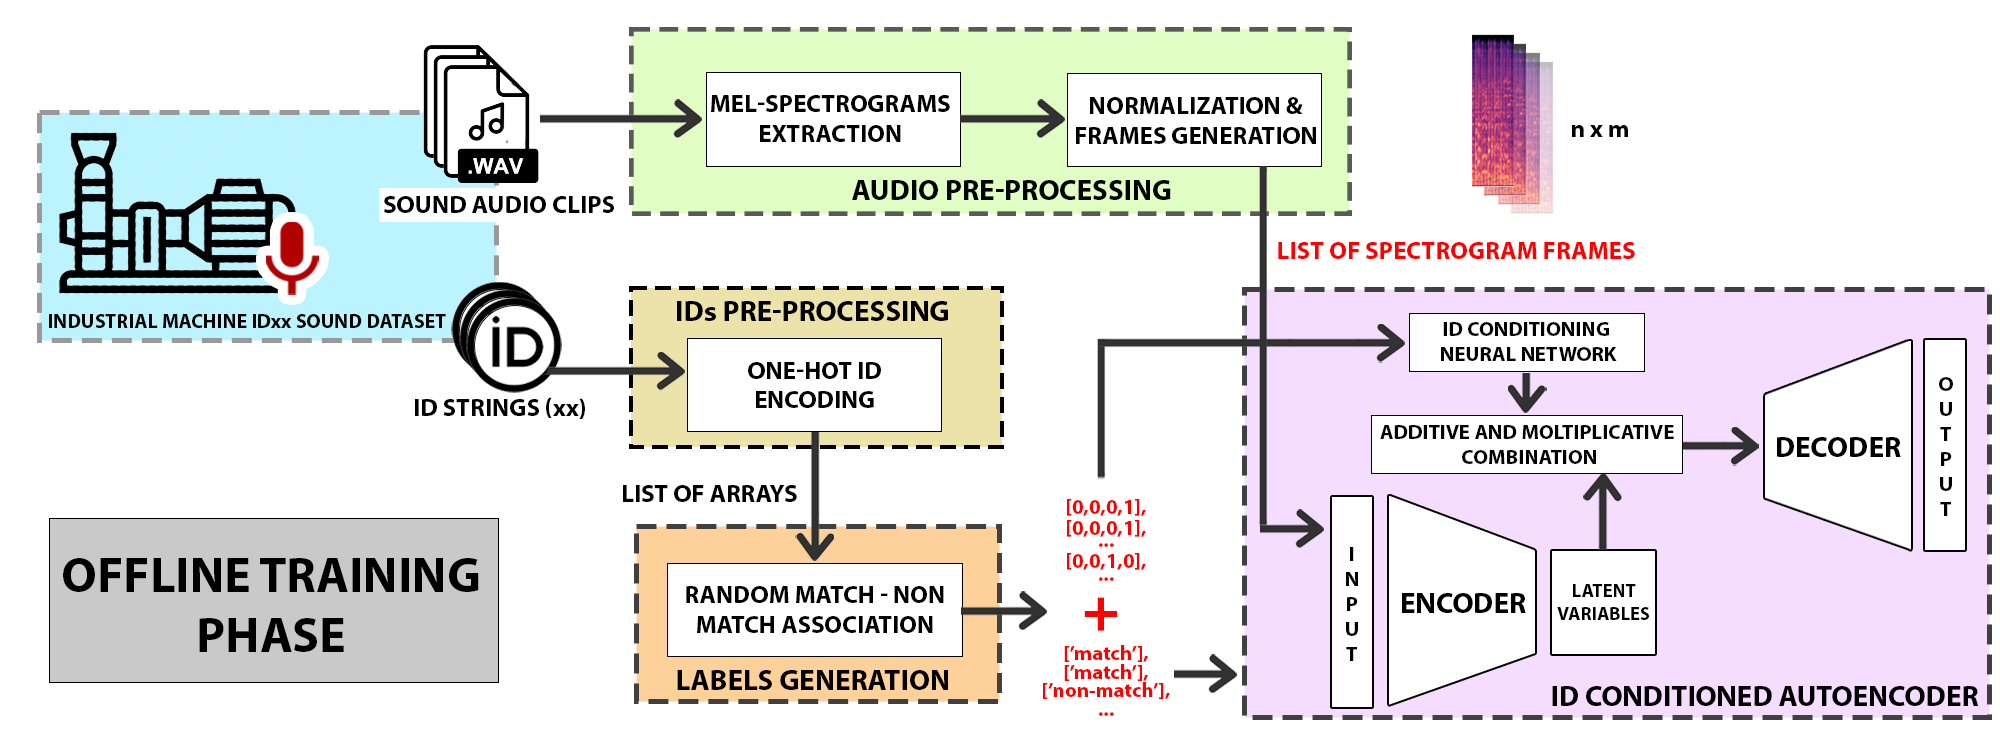
\includegraphics[scale=0.48]{TESI DI FIORE/img/offline-architecture.png}
\centering
\caption{Overview of offline training phase of the proposed ASD system.}
\label{offline-asd-system}
\end{figure}
This part of the overall architecture is responsible of the autoencoder training. The training process must be done in offline manner with the use of a pre-collected normal audio clips which belong to the machine that is under observation. In addition to the dataset, different other components can be noticed analyzing the Figure \ref{offline-asd-system}: the Features Extraction block, the IDs Pre-Processing block, the Label Generation block and finally the ID Conditioned Autoencoder. The first three parts prepare the dataset for training process, which it is executed in the last one.
\subsubsection{Dataset Structure}
In addition to the audio clips, the dataset must provide the ID used to identify the particular kind of $M$, embedding it into clips' filename (with \textit{.wav} extension) or in a separated file (obviously maintaining a one-to-one correspondence with audio files). Definitely, the data should be structured in couples composed by audio clips plus a numerical identifier.
\subsubsection{Offline Features Extraction}
This part of the architecture is responsible of the transformation of audio clips, an operation that is needed to make them ready for the neural network learning process. There are two different components in this block and they are the Mel-Spectrogram Extractor and the Frame Generator:
\begin{itemize}
    \item {\textit{Mel-Spectrogram extractor} receives in input the audio clips and it produces in output the corresponding spectrograms in a log-mel-scale.}
    \item {\textit{Frame generator} produces in output a segmentation in $n \times m$ overlapping frames of the received log-mel-spectrograms.  }
\end{itemize}
A little digression should be made about what these spectrograms are and how the first block calculate them. A signal is a variation in a certain quantity over time and for audio, this quantity is air pressure, sampled by microphones with a particular rate (in the order of kHz). The Fast Fourier Transform (FFT) is an algorithm that allows the decomposition of a signal into its individual frequencies and the frequency’s amplitude, converting it from the time domain into the frequency domain (the spectrum). The Short-Time Fourier Transform (STFT) allows the representation of the spectrum of these signals as they vary over time (the spectrogram). As audio signals' frequency content vary over time (non-periodic signals) STFT is applied. In particular, the STFT is a FFT computed on overlapping windowed segments of the signal (Figure \ref{sftf}).\\
\begin{figure}[ht]
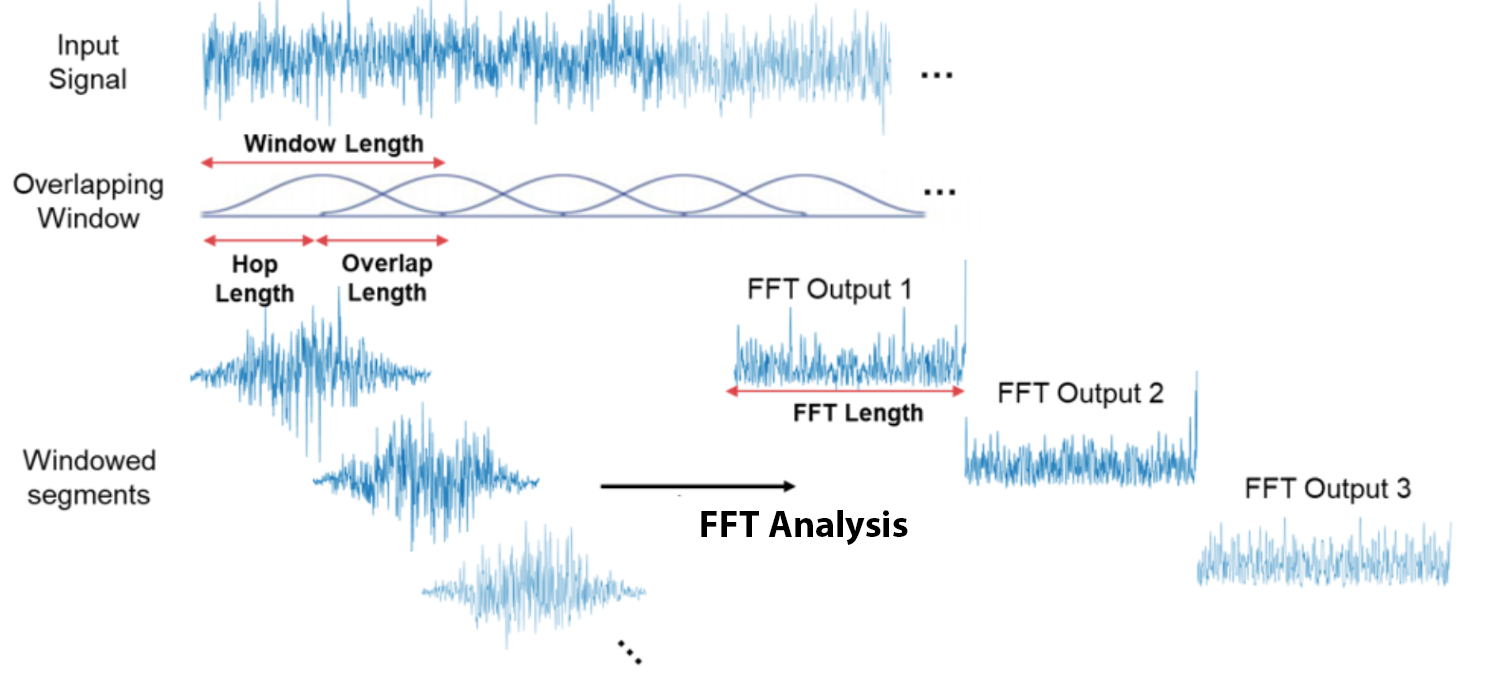
\includegraphics[scale=0.4]{TESI DI FIORE/img/STFT.png}
\centering
\caption{Overview of the STFT process.}
\label{sftf}
\end{figure}
Spectrograms usually presents on the x-axis the time, on the y-axis the frequencies and the amplitude is indicated by colors. Log-mel-spectrograms are spectrograms in which the frequencies on y-axis are represented using the Mel-Scale (seen in the previous chapter) and the amplitudes are expressed in Decibel (dB). The most important parameters involved into this transformation process are the length of the window used for STFT ($n\_fft$), the length of the overlap between two successive windows ($hop\_length$) and the number of bins used for the transformation into the Mel scale ($n$).
In the Figure \ref{features-extraction} a complete graphical view of what this block does is illustrated.
\begin{figure}[ht]
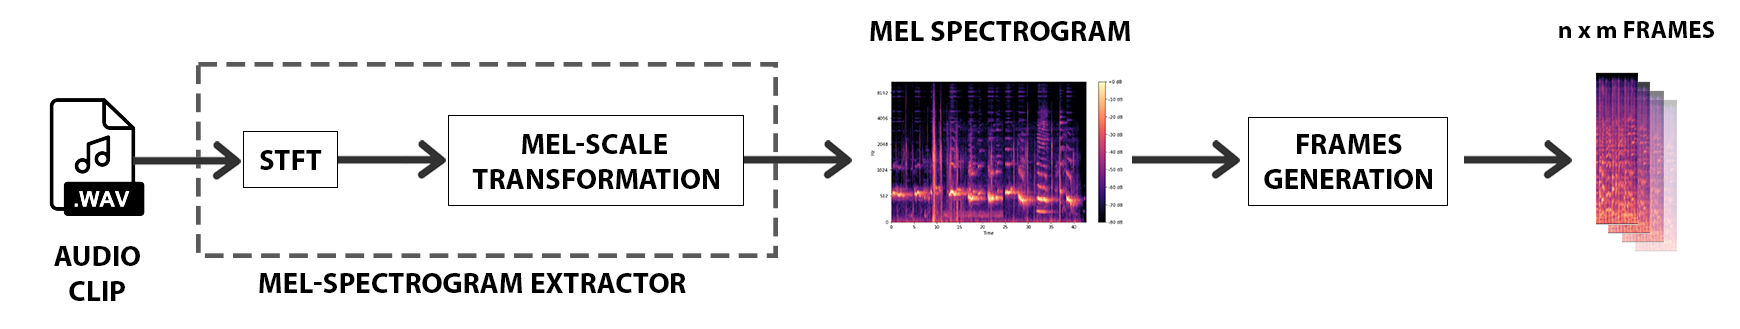
\includegraphics[scale=0.8]{TESI DI FIORE/img/FeatureExtraction.png}
\centering
\caption{Features extraction block}
\label{features-extraction}
\end{figure}
In the offline phase, $n \times m$ frames are generated from all $n \times q$ spectrograms of the training set, in order to build a new, pre-processed dataset ready for training process.
\subsubsection{IDs Pre-Processing}
This block receives in input a string (the machine ID), associated to each audio clip and converts it to a binary sequence, whose length depends by the number of different kinds of $M$. This is done by the One-Hot Encoder. One-hot encoding is a technique used to convert some categorical or nominal features in order to make them compatible with training algorithm. Here ID strings are converted. Let's take an example. Suppose that there is a machine $M$ and suppose that there are four type of $M$, identified as $ID00$, $ID01$, $ID02$, $ID03$. The one-hot encoder converts them to $[0,0,0,1]$, $[0,0,1,0]$, $[0,1,0,0]$ and $[1,0,0,0]$, respectively. This operation arranges the IDs to be the input of the ID Conditioning Neural Network, better explained in the next sections. In conclusion, because of each audio file spectrogram is segmented in frames, this block must ensure that each frame of the same spectrogram are associated to the same binary sequence.
\subsubsection{ID Conditioned Autoencoder}
This part of the architecture is obviously the most important one. It receives in input two lists: the list of spectrogram frames and a list of one-hot-encoded ID arrays. The list of strings from Label Generation is used for the loss calculation during the training process, so that it is not a real input of the neural network. In this block there are two main components: the autoencoder, composed by an encoder and a decoder, which receives the spectrogram frames in input and the ID Conditioning Neural Network, which receives ID arrays. Following there is a mathematical representation these components \cite{18IDConditionedAutoEncoder}:
\begin{itemize}
    \item {Encoder $E: \mathcal{X} \rightarrow \mathcal{Z}$ which maps the input $X$ into its encoded version $Z = E(X)$;}
    \item {Decoder $D:  \mathcal{Z} \rightarrow \mathcal{X}$ which takes the code from $\mathcal{Z}$ and outputs an reconstruction of $X$; }
    \item {Conditioning made by two functions $H_\gamma$ and $H_\beta: \mathcal{Y} \rightarrow \mathcal{Z}$, taking in input the one-hot encoded ID $l$ from $\mathcal{Y}$ in order to map it into $H_\gamma(l)$ and $H_\beta(l)$, with the same size as code from $\mathcal{Z}$.}
\end{itemize}
The encoder and the decoder can be created with different type of layers, like convolutional, LSTM or fully-connected layers. The layer in between the encoder and the decoder is a latent or encoded representation of the input $X$, or else $Z$. Differently from conventional autoencoders, in this architecture decoder's input is not $Z$, but its mathematical combination with the output of conditioning functions: $H(Z,l) = H_\gamma(l) \cdot Z + H_\beta(l)$. The conditioning functions can be realized, for example, using dense layers and activation functions. In conclusion the output of the entire autoencoder is $D(H(E(X),l))$.
\subsubsection{Label Generation}
The goal of ID embedding is to inform the model about the presence of different kinds of machine $M$, for the recognition of their different normal behaviours. In general, anomalous sound of a machine $M$ with ID $x$ could be similar to normal sound of machine $M$ with ID $y$ and this could generate some false negative (FN), because the autoencoder is unable, in this case, to distinguish this anomalous behaviours from normal one on which it has been trained on. The key concept is that the autoencoder must be trained to reconstruct normal audio spectrograms in input only if the provided ID is correct. With this assumptions, after the training, if a normal test sample is placed in input, a low reconstruction error (in terms of mean absolute error or mean squared error) is expected, while if there is an anomalous one, an high  reconstruction error is generated, even if this anomalous behavior is similar to a normal behaviour of another machine. The similarity problem is so resolved by the presence of the ID. At this point a question arises: the only ID conditioning is it sufficient for this task? The answer is no and for this reason there is the Label Generation block. This block randomly changes with a probability $1-\alpha$ the correct ID binary sequence associated to an audio clip to another one available and it adds, for each frame associated to the same audio clip, the string \textit{match} or \textit{not-match} on the basis of the decisions. For example if there are 100 audio clips and $\alpha$ is 0.75, 75 audio clips will be associated to the correct ID sequence, the remaining 25 will be associated to a random one, from those available (so that the frame belonging to the same spectrogram have the same ID binary sequence and the same string). Moreover, in order obtain what it is just described, a new loss must be tuned because the classical difference between the encoder input and the decoder output is not enough. In fact, to allow a good reconstruction of the input only when the ID is correct, during the training, if the label is \textit{match} the loss function must be calculated in classical way as $||D(H(E(X),l)) - X||$
while if the label is \textit{not-match} the loss function must be calculated using an arbitrary value C: $||D(H(E(X),l)) - C||$.
In conclusion, when the input spectrogram frames are associated to wrong IDs, the autoencoder tries to reconstruct C (and so high reconstruction error).
\subsection{Online Operation Phase}
\begin{figure}[ht]
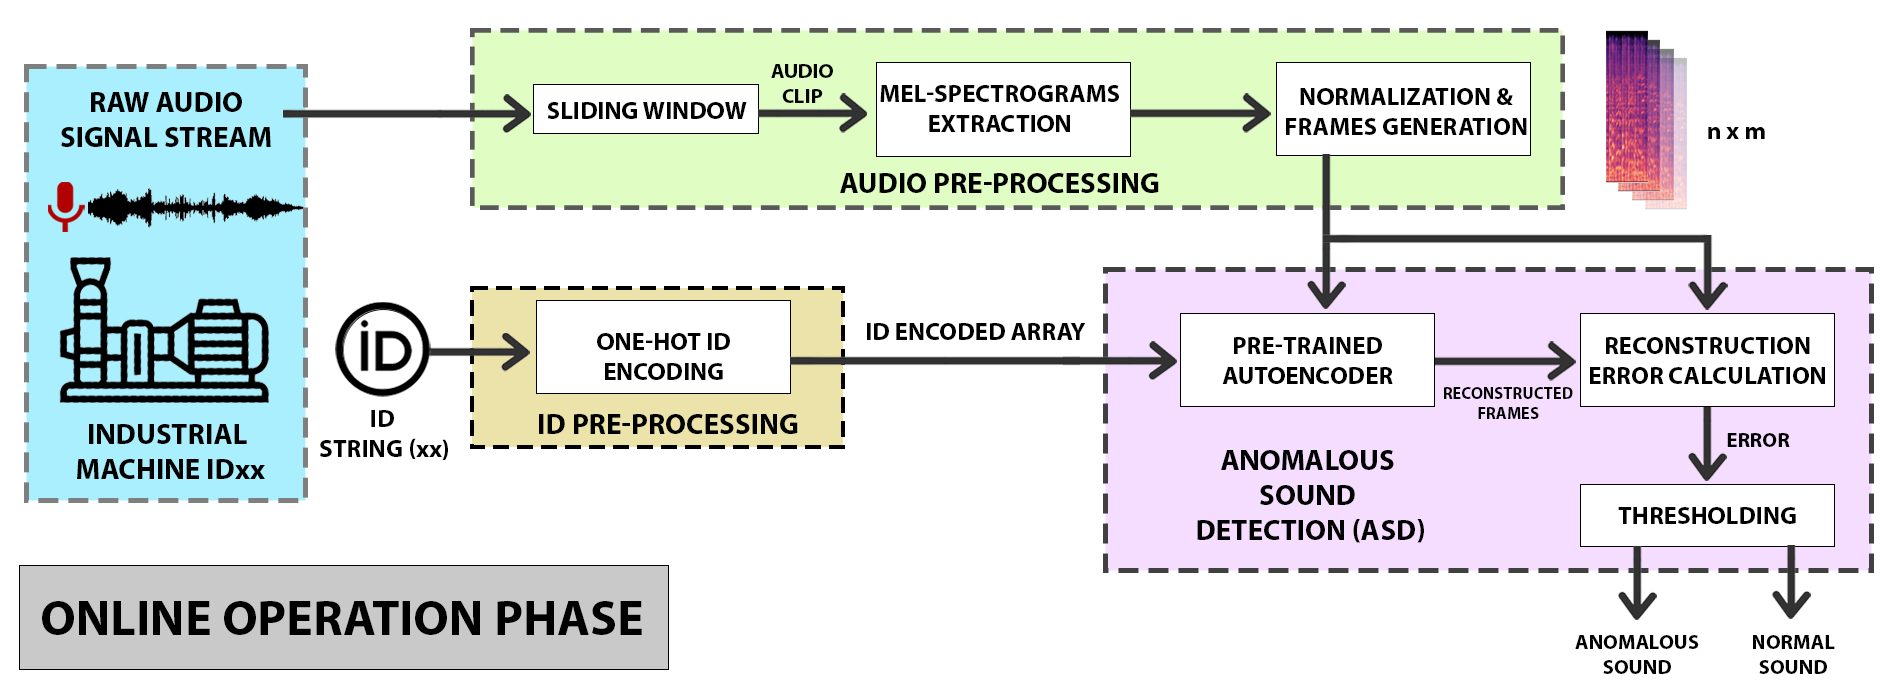
\includegraphics[scale=0.45]{TESI DI FIORE/img/online-architecture.png}
\centering
\caption{Overview of online operating phase of the proposed ASD system.}
\label{online-asd-system}
\end{figure}
The architecture used for online operation phase is very similar to the part just described, except for few components. The first thing that must be noticed is that this part of the architecture is meant for an effective and an operative use on field, since the left part of the Figure \ref{online-asd-system} shows that there is not a dataset but there is the real time raw audio stream from microphones disposed around the machine $M$. As other elements have been already explored in previous sections, following  there is a description of Feature Extraction block and the Anomalous Sound Detection block. 
\subsubsection{Online Feature Extraction}
It is very similar to the one presented before, with exception of the sliding window component. Because of real-time anomaly detection, there are not audio files, but there is a continuous audio stream. The autoencoder model is implemented and trained to work with $T$ seconds audio clips. For this reason, the sliding window component takes in input the stream and samples the last $T$ seconds from it, every $h$ seconds. Next, the audio clip obtained passes into mel-spectrogram extractor and into the frame generator, already presented. 
\subsubsection{Anomalous Sound Detection}
This is the final block of the online architecture and the one that is responsible of the sound labeling as normal or anomalous. In this part three components are highlighted: the pre-trained autoencoder, the reconstruction error calculator and a threshold. The pre-trained autoencoder is the result of the operations made by the offline part of the architecture. The reconstruction error calculator takes in input the output of the autoencoder and its input in order to evaluate the difference between these two (as the loss calculation during the training phase). This operation is made for each frame of the spectrogram associated to the audio clip and then an average of recostruction errors is calculated for the comparison with the threshold. In fact, the threshold is used to establish if the average reconstruction error is high enough to classify clips as anomalous. It could be chosen using reconstruction errors of training samples.
\section{Hyperparameters}
In order to give a better idea related to the hyperparameters of the proposed model, following there is a summary of the most important ones:
\begin{itemize}
    \item {\textit{C}: the constant vector that must be reconstructed by the autoencoder when the provided ID is wrong;}
    \item {$\alpha$: the percentage of correct frame-ID couples in training set;}
    \item {\textit{NUM\_CONDITIONING\_LAYERS}: number of layers of the conditioning neural network;}
    \item {\textit{NUM\_CONDITIONING\_NEURONS}: number of neurons used in the the conditioning layers of the neural network and also the dimension of the encoded input generated by the encoder.}
\end{itemize}
Clearly, because of the architecture is compatible with different kinds of autoencoder layers, other hyperparameters that should be taken in consideration are whose that arise from them. Moreover, there are other hyperparameters, such as learning rate, batch size and number of epochs, which are not dependent on the proposed architecture but affect the training stage of the model.
\section{Implementation technologies}
In this section, some implementation details about the proposed model are given. The model was implemented in Python 3. Used technologies and libraries are:
\begin{itemize}
    \item {Google Colab: Colab notebooks are Jupyter notebooks that run in the cloud and are highly integrated with Google Drive, making them easy to set up, access, and share;}
    \item {Tensorflow: it is an end-to-end open source platform for Machine Learning;}
    \item {Keras: it is an open source Deep Learning API written in Python3;}
    \item {NumPy, used to work in an efficient way with arrays;}
    \item {SciKit-Learn, a machine learning library, containing simple and efficient tools for predictive data analysis;}
    \item {Librosa, a Python library for audio and music processing.}
\end{itemize}

